\begin{frame}{Paper 1: ILP vs DL in One-Shot Learning}

\begin{itemize}
\vfill
    \item Title: "Human-like rule learning from images using one-shot hypothesis derivation"
\vfill
    \item Author: Muggleton
\vfill
    \item Content: ILP vs Deep Learning in One Shot Learning
\vfill
    \item Databases: 
    \begin{itemize}
        \item Omniglot dataset: character recognition
        \item UK Biobank: neurodegenerative disease identification
    \end{itemize} 
\vfill
    \item Link: \url{https://www.researchgate.net/publication/355875180_Human-like_rule_learning_from_images_using_one-shot_hypothesis_derivation}
\vfill
\end{itemize}
    
\end{frame}

\begin{frame}{Omniglot Dataset}

\begin{minipage}{0.7\textwidth}%\raggedleft
    \begin{itemize}
        \item Character recognition
        \item 1623 different handwritten characters from 50 different alphabets
        \item Each character is a different class
        \item Each character has 20 examples
        \begin{itemize}
            \item[\ding{43}] Written by 20 different people 
        \end{itemize}
    \end{itemize}
\begin{figure}
    \centering
    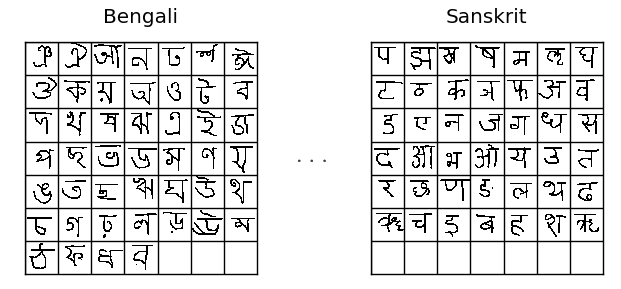
\includegraphics[scale=0.3]{images/Omniglot - Alphabets.png}
\end{figure}
\end{minipage}
\hfill
\begin{minipage}{0.2\textwidth}%\raggedleft
\begin{figure}
    \centering
    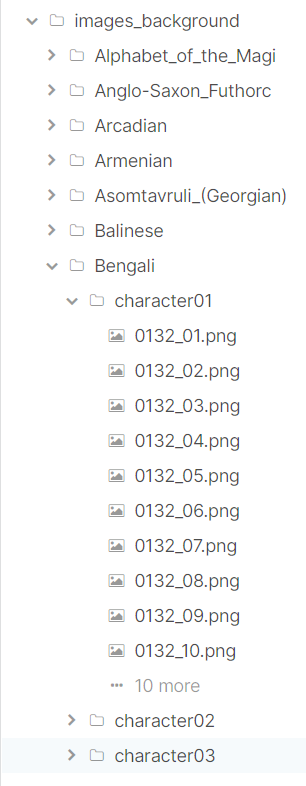
\includegraphics[scale=0.25]{images/Omniglot Dataset.png}
\end{figure}
\end{minipage}

\end{frame}

\begin{frame}{One Shot Learning}

\begin{itemize}
    \item Classification task in which one is provided with 1 (or few) example of each class
    \item Deep learning usually needs thousands of examples to learn a new class
    \item Human only need to see a picture of a giraffe once to be able to recognise another one
    \item Most well known use case: Facial recognition
\end{itemize}    
\begin{figure}
    \centering
    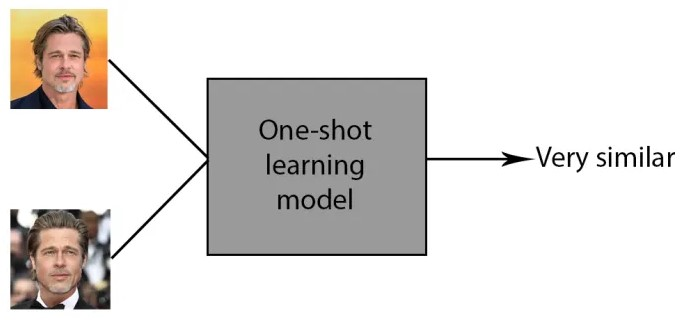
\includegraphics[scale=0.4]{images/imagerecog.jpg}
\end{figure}

\end{frame}

\begin{frame}{Siamese Neural Networks}

\begin{itemize}
\item Model trained to differentiate between images of different classes 
\item \url{https://www.cs.cmu.edu/~rsalakhu/papers/oneshot1.pdf}  
\end{itemize}

\begin{figure}
    \centering
    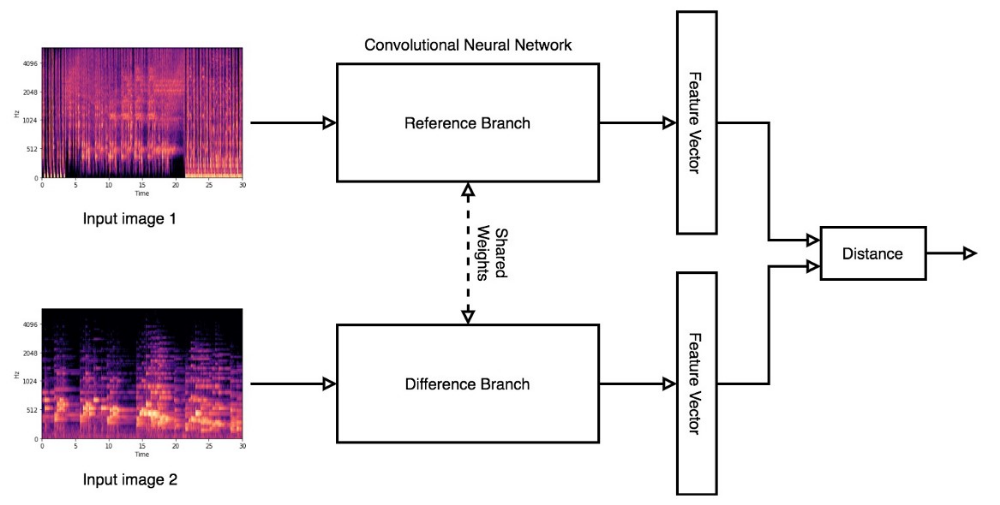
\includegraphics[scale=0.18]{images/siamese.png}
    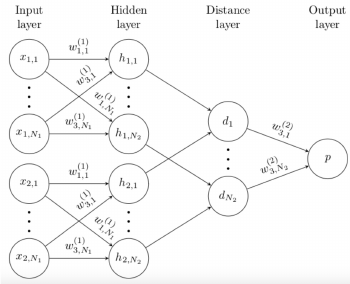
\includegraphics[scale=0.6]{images/siamese2.png}
    \caption{Architectures of a Siamese NN}
\end{figure}

\end{frame}

\begin{frame}{ILP approach}
\begin{itemize}
    \item One-Shot Hypothesis Derivation (OSHD) based on \item Implemented in Toplog
    \item Background knowledge:
    \begin{figure}
        \centering
        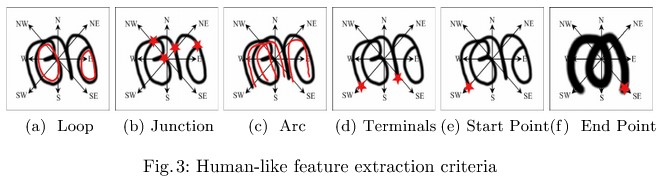
\includegraphics[scale=0.4]{images/ilpfeatureextraction.jpg}
        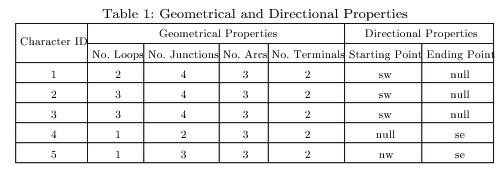
\includegraphics[scale=0.4]{images/geomtable.jpg}
    \end{figure}    
    \item Modes:
    \begin{figure}
        \centering
        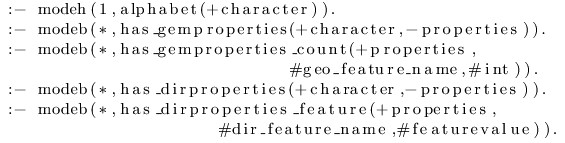
\includegraphics[scale=0.4]{images/modes.jpg}
    \end{figure}
\end{itemize}
\end{frame}

\begin{frame}{ILP vs DL}

Background
\begin{itemize}
    \item ILP:
    \begin{itemize}
        \item Modes
        \item Table of Geometrical and Directional Properties
    \end{itemize}
    \item DL:
    \begin{itemize}
        \item Many examples to train the model 
        \item 40 (of 50) alphabets used as background
    \end{itemize}
\end{itemize}

Training
\begin{itemize}
    \item ILP:
    \begin{itemize}
        \item The 1 example generates a new rule
    \end{itemize}
    \item DL:
    \begin{itemize}
        \item The 1 example is kept in memory
    \end{itemize}
\end{itemize}

Testing
\begin{itemize}
    \item ILP:
    \begin{itemize}
        \item The new example is verified against the new rule
    \end{itemize}
    \item DL:
    \begin{itemize}
        \item The new example, with the training example are compared to see whether they belong to the same class
    \end{itemize}
\end{itemize}
    
\end{frame}

\begin{frame}{Results}

\begin{itemize}
    \item Results provided by Muggleton are not consistent with those provided by the original Siamese paper
\end{itemize}

\begin{figure}
    \centering
    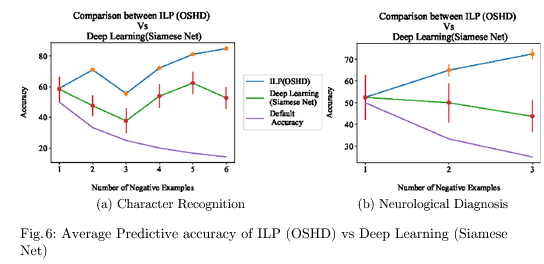
\includegraphics[scale=0.45]{images/SiameseNN v ILP.png}
    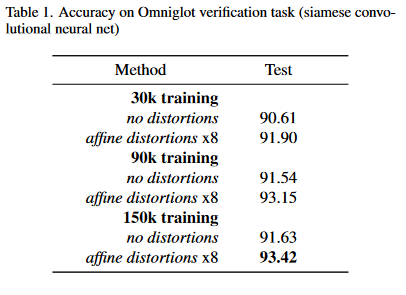
\includegraphics[scale=0.45]{images/Accuracy SiameseNN.png}
    \caption{Comparison of the two models by Muggleton (left) and accuracy in the Siamese paper (right)}
\end{figure}    
    
\end{frame}

\begin{frame}{Approach 2: DeepProbLog}

\begin{itemize}
\vfill
    \item Title: "From Statistical Relational AI to
Neural Symbolic Computation: DeepProbLog"
\vfill
    \item Author: Luc De Raedt
\vfill
    \item Content: Adding a ProbLog brick at the end of Neural Networks
\vfill
    \item Databases: 
    \begin{itemize}
        \item MNIST dataset: digit recognition
    \end{itemize} 
\vfill
    \item Link: \url{https://www.i-aida.org/wp-content/uploads/2022/03/Luc-De-Raedt_compressed.pdf}
\vfill
\end{itemize}
    
\end{frame}

\begin{frame}{DeepMNIST addition}
    
\begin{itemize}
    \item Set of examples:
    \begin{figure}
        \centering
        
\includegraphics[scale=0.35]{images/DeepProbLog - Examples.jpg}
    \end{figure}
    \item Model:
    \begin{itemize}
        \item Neural network:
        \begin{figure}
            \centering
            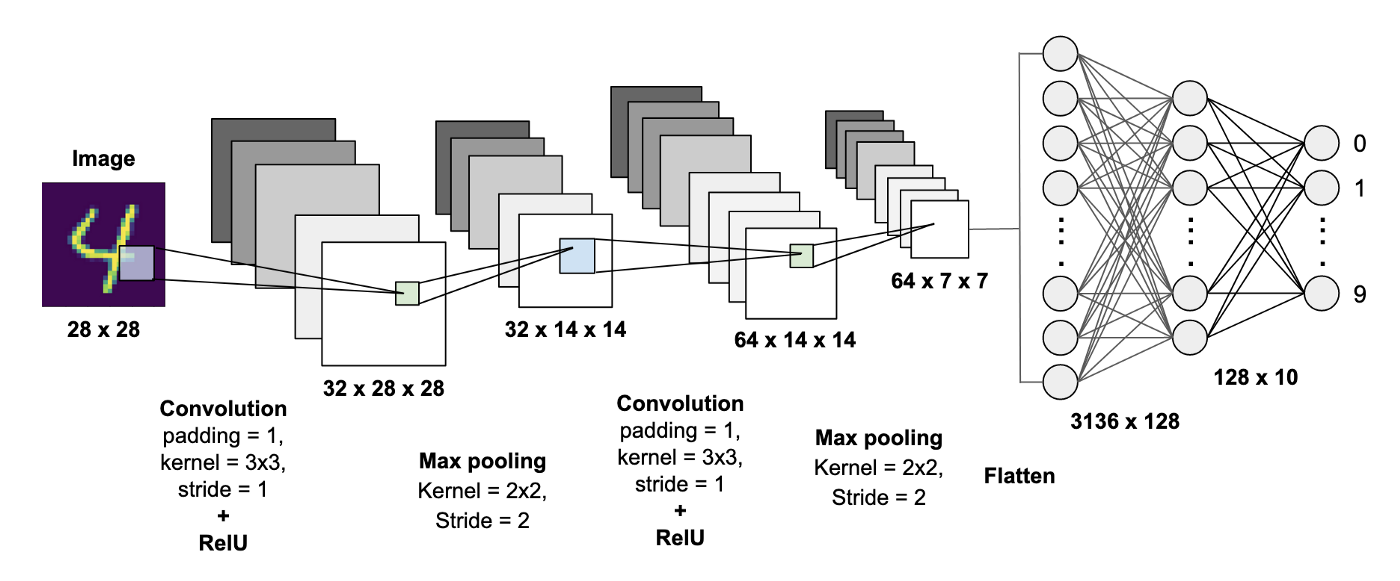
\includegraphics[scale=0.1]{images/ExampleOfNN.png}
        \end{figure}
        \item ProbLog brick:
    \begin{figure}
        \centering
        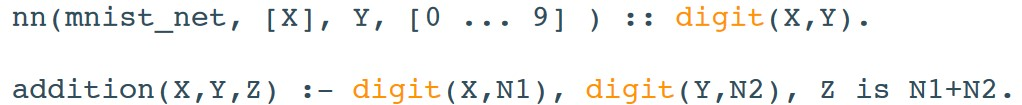
\includegraphics[scale=0.3]{images/ProbLog brick.jpg}
    \end{figure}
    \end{itemize}
    \item Execution:
    \begin{figure}
        \centering
        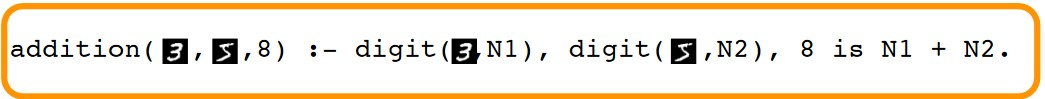
\includegraphics[scale=0.3]{images/3+5 example.jpg}
    \end{figure}
\end{itemize}    

\end{frame}

\begin{frame}{Frame Title}
    
\end{frame}